\section{Results}

The two frontline occupations (Social and Human Service Assistants and Child, Family and School Social Workers) have little of their working day exposed to AI. The managerial occupation Social and Community Service Managers shows more direct exposure to AI. In all three occupations studied, the greater share of exposure is indirect, meaning that LLMs could support the task if dedicated software were built to support it. The following sections present working time in each exposure category (4.1), compare time-weighted vs task-weighted exposure (4.2), describe observed patterns of LLM use (4.3), and present exposure results at the scale of the workforce.

\subsection{Exposed working time}

Social and Human Service Assistants spend about 24 minutes per day on tasks that could be classified as directly exposed to AI (Figure 1). That directly exposed time is spread across six small tasks, the largest being referring clients to other agencies (10 minutes per day) and submitting reports to a supervisor (9 minutes per day). A further 2 hours, 51 minutes per day fall on three tasks that are exposed only with additional software: developing care plans (1 hour, 48 minutes), locating housing (32 minutes), and keeping records of client visits (31 minutes). The remaining 3 hours 45 minutes, more than half the 7-hour workday, are not exposed. These include assessing client needs, supervising group activities, and interviewing families.

\begin{figure}[!htbp]
\centering
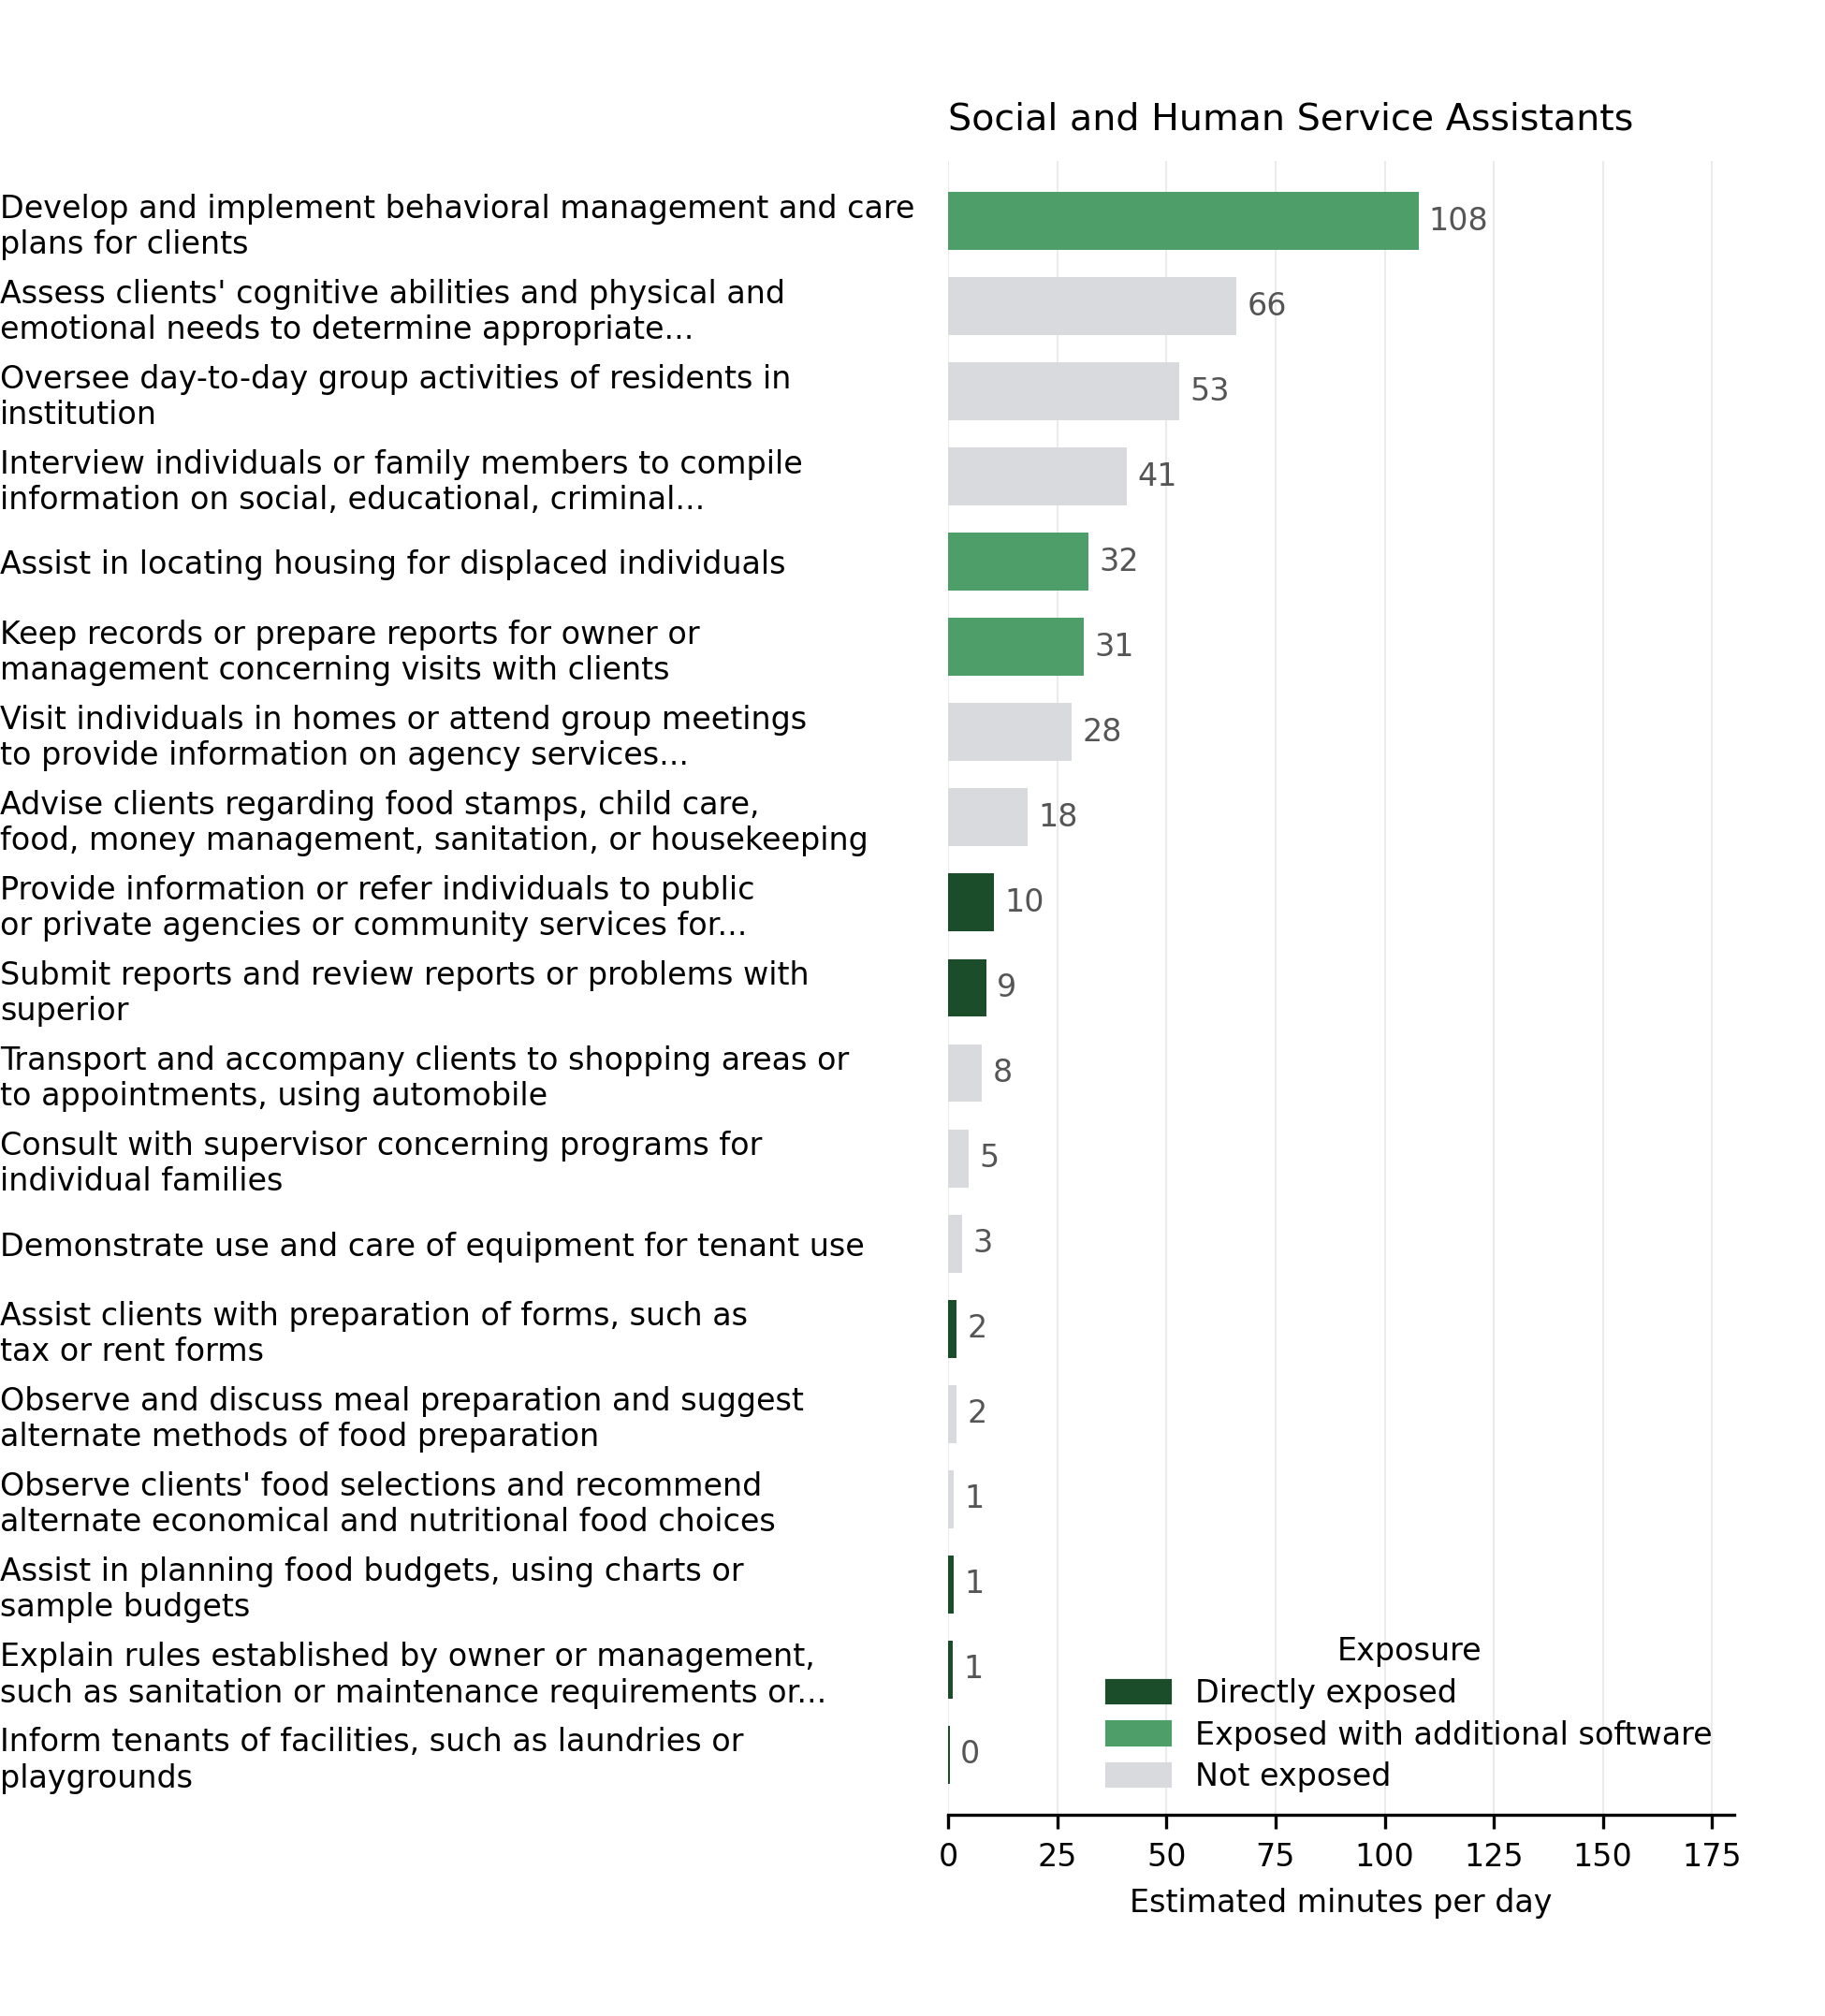
\includegraphics[width=0.8\textwidth]{figures/fig1_assistants.png}
\caption*{Figure 1: Theoretical task-based exposure to AI for Social and Human Service Assistants. Ratings are human ratings from Eloundou et al. (2024); hours from Hatgis-Kessell et al. (2026).}
\end{figure}

Child, Family, and School Social Workers show a similar pattern (Figure 2). The total amount of time a worker spends on directly exposed tasks is about 36 minutes per day. One task, "Counsel students whose behavior, school progress, or mental or physical impairment indicate a need for assistance, diagnosing students' problems and arranging for needed services" takes up 26 of those directly exposed minutes. Time on partially exposed tasks take an additional 1 hour 58 minutes and include counseling individuals and families (39 minutes), maintaining case records (35 minutes), and advising parents (27 minutes). The majority of the day (4 hours 27 minutes) is not exposed, including the most time-consuming task for this occupation, ``Placing children in foster or adoptive homes, institutions, or medical treatment centers'' (1 hour 28 minutes).

\begin{figure}[!htbp]
\centering
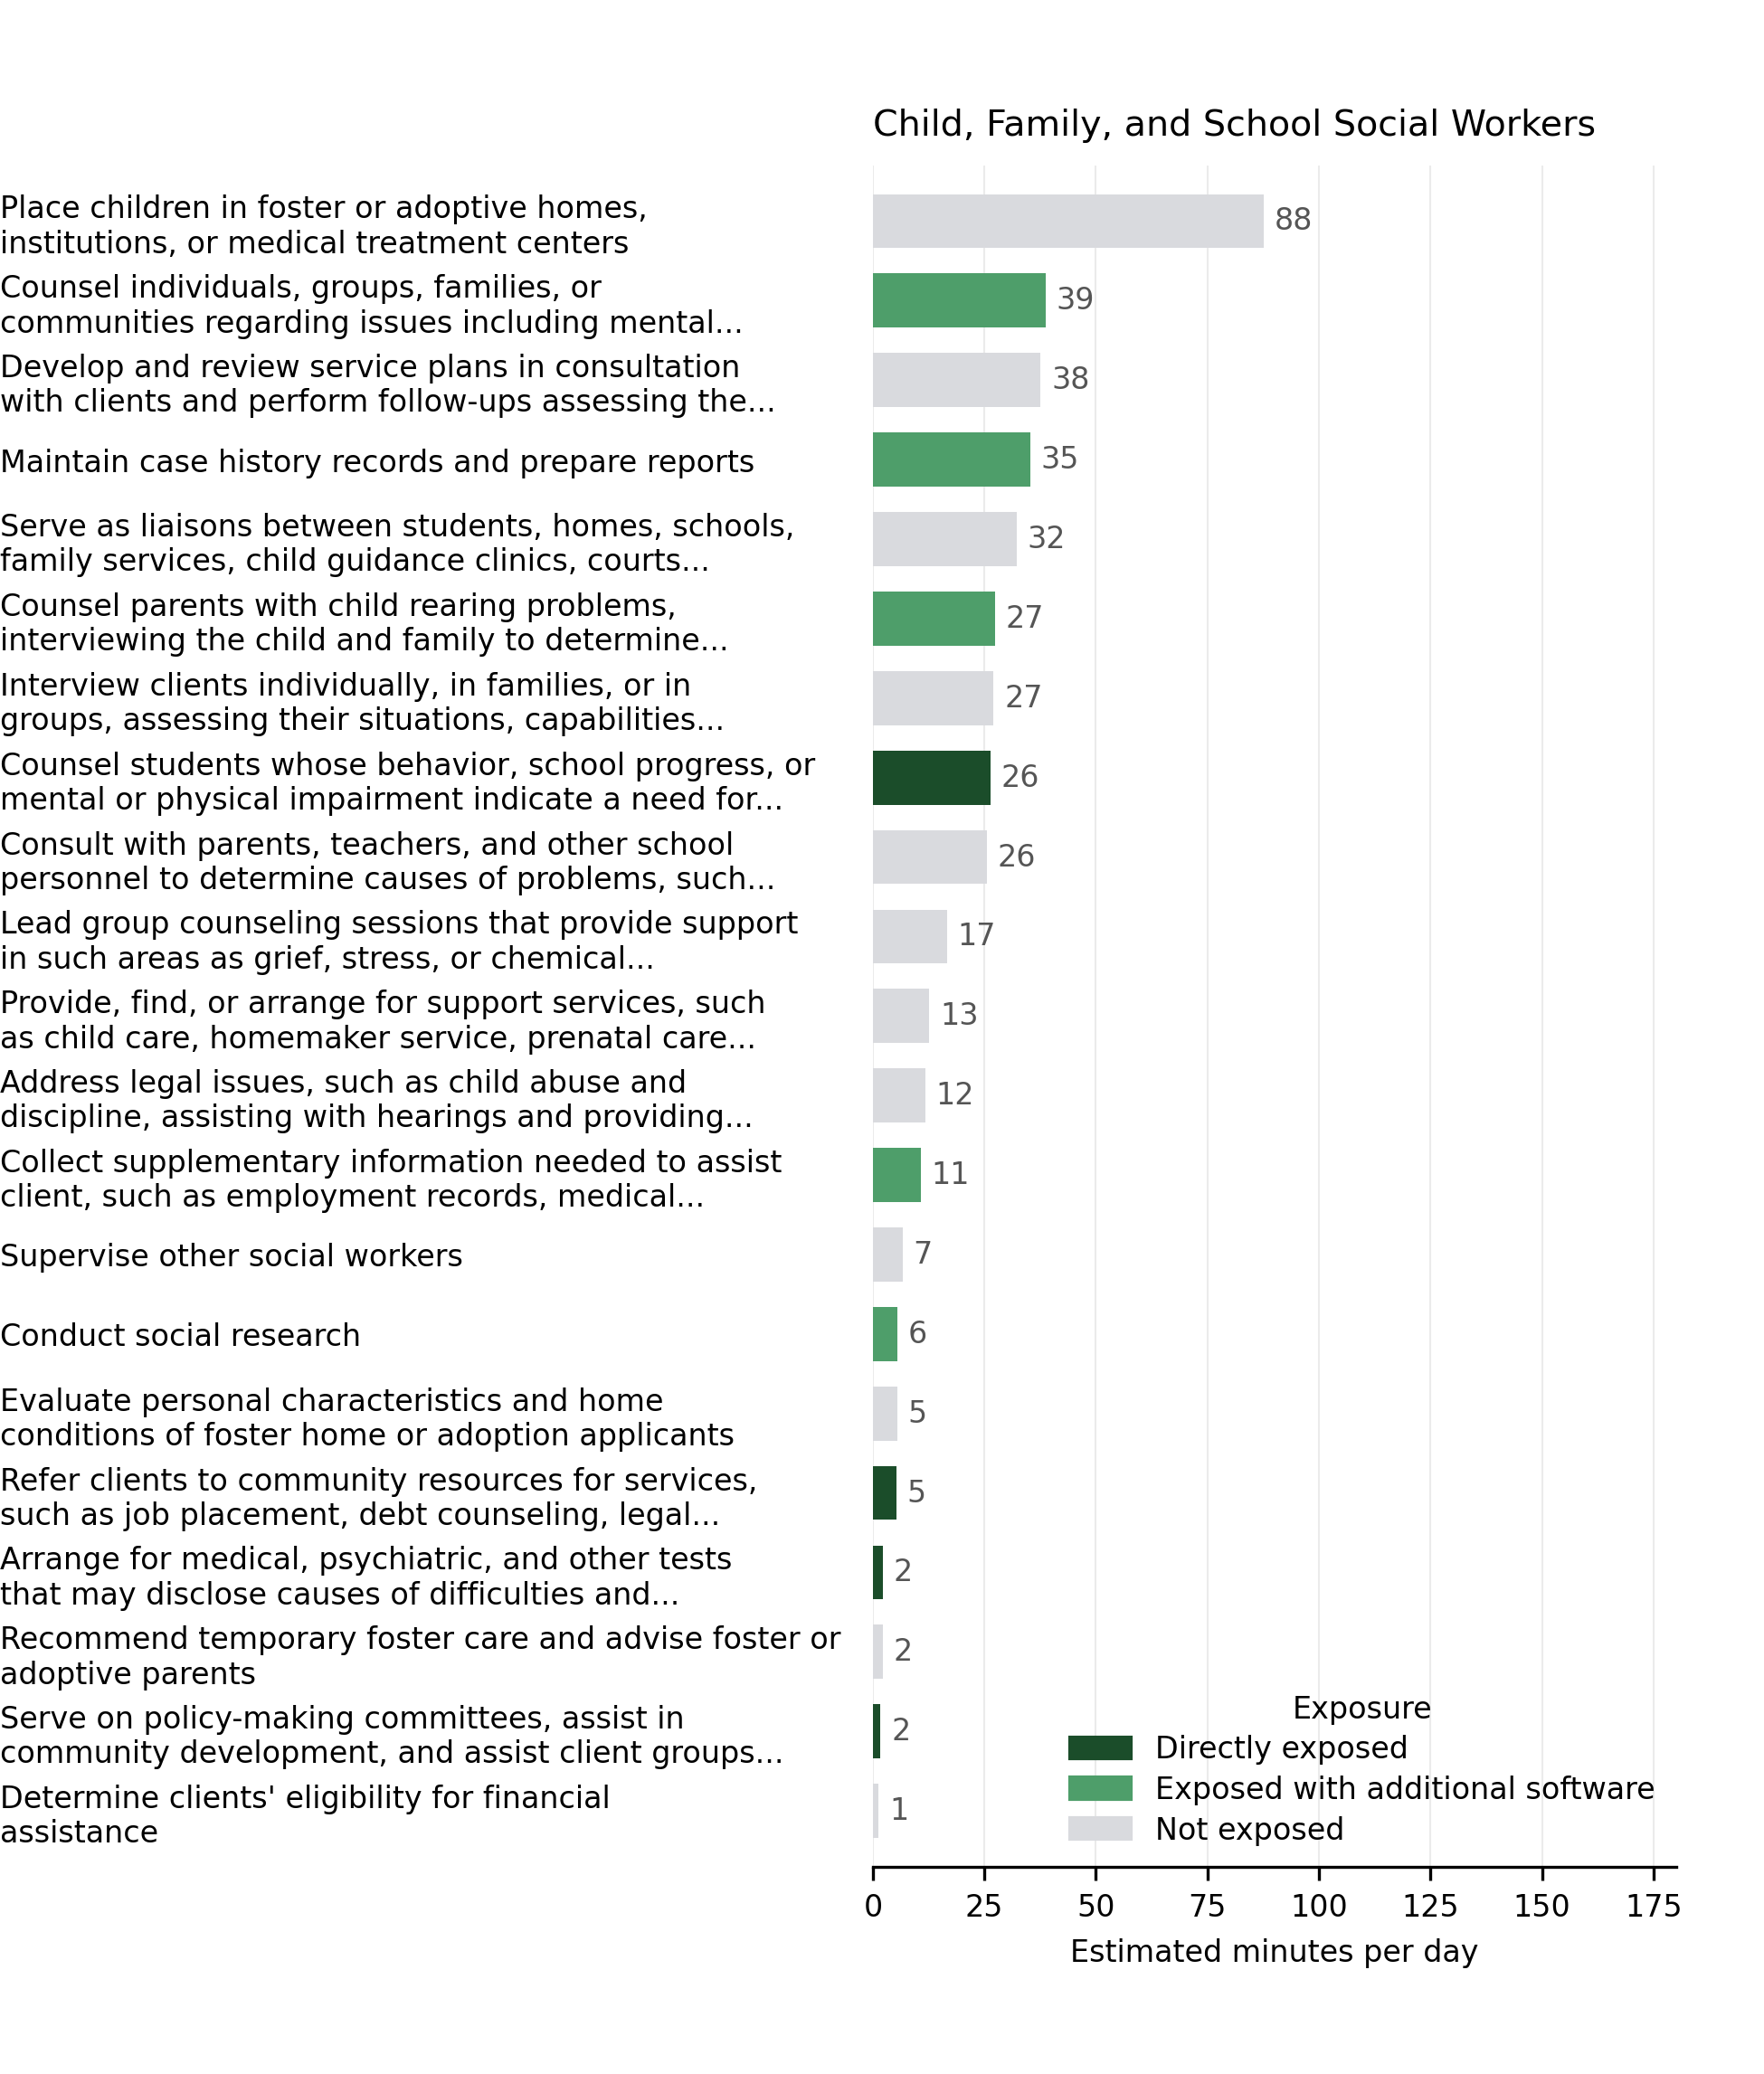
\includegraphics[width=0.8\textwidth]{figures/fig2_social_workers.png}
\caption*{Figure 2: Theoretical task-based exposure to AI for Child, Family, and School Social Workers. Ratings are human ratings from Eloundou et al. (2024); hours from Hatgis-Kessell et al. (2026).}
\end{figure}

Social and Community Service Managers show a different pattern from the two frontline occupations (Figure 3). Managers spend about a quarter of their workday (1 hour 41 minutes) directly exposed tasks. These tasks include establishing administrative procedures (49 minutes) and participating in determining organizational policy (21 minutes). An additional 3 hours 52 minutes of the managers 7-hour workday is considered partially exposed, of which one task, "Implement and evaluate staff, volunteer, or community training programs" accounts for 2 hours 51 minutes of this time. Only 1 hour 27 minutes of the managers' workday is considered not exposed.

\begin{figure}[!htbp]
\centering
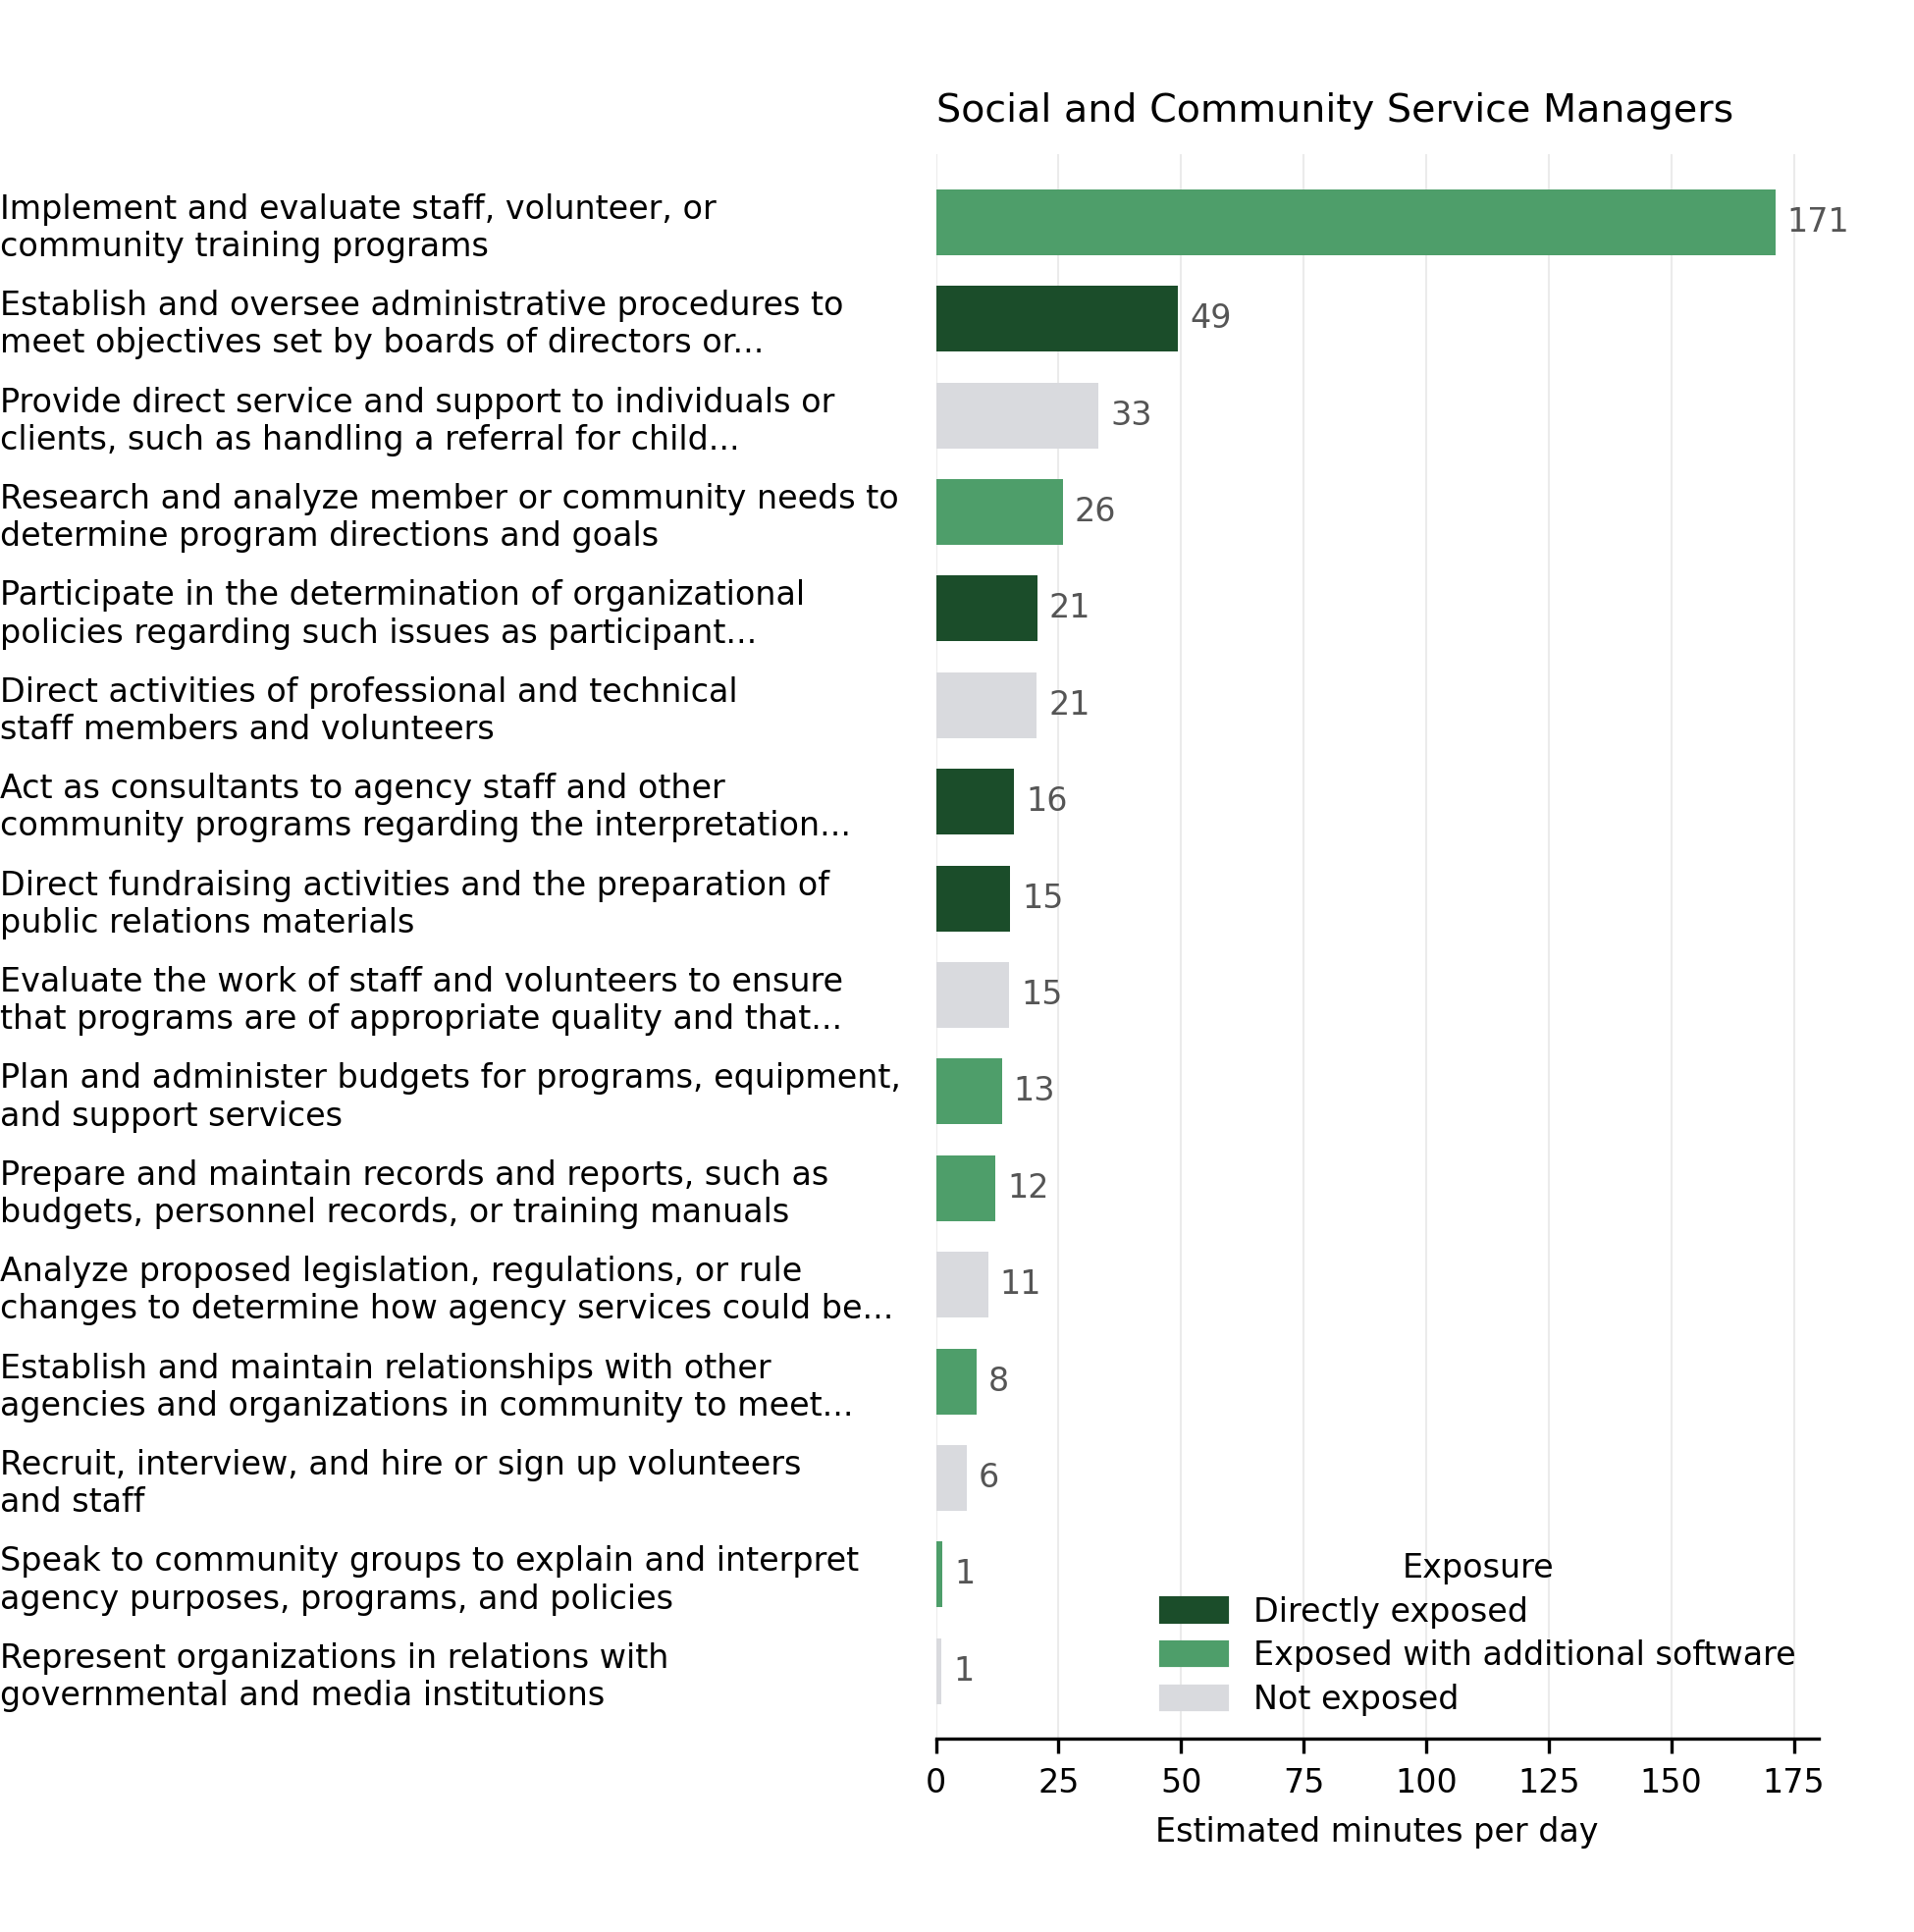
\includegraphics[width=0.8\textwidth]{figures/fig3_managers.png}
\caption*{Figure 3: Theoretical task-based exposure to AI for Social and Community Service Managers. Ratings are human ratings from Eloundou et al. (2024); hours from Hatgis-Kessell et al. (2026).}
\end{figure}

Job exposure to AI for each of the three occupations studied is summarized in Table 3. Managers have the most directly exposed time at 1 hour 41 minutes per day, while the two frontline workers show 24 and 36 minutes per day of directly exposed work. For all three occupations, time exposed only with additional software exceeds directly exposed time.

\begin{table}[!htbp]
\tablesize
\caption*{\textbf{Table 3.} Daily working time by exposure category.}
\begin{tabularx}{\textwidth}{@{}>{\raggedright\arraybackslash}X >{\raggedright\arraybackslash}p{2.5cm} >{\raggedright\arraybackslash}p{3.6cm} >{\raggedright\arraybackslash}p{2.3cm}@{}}
\toprule
& Time directly exposed (E1) & Time exposed with additional software (E2) & Time not exposed (E0) \\
\midrule
Social and Human Service Assistants & 0:24 (6\%) & 2:51 (41\%) & 3:45 (54\%) \\
Child, Family, and School Social Workers & 0:36 (8\%) & 1:58 (28\%) & 4:27 (64\%) \\
Social and Community Service Managers & 1:41 (24\%) & 3:52 (55\%) & 1:27 (21\%) \\
\bottomrule
\end{tabularx}
\tablenote{\emph{Note:} Time per 7-hour day in hours and minutes, with share of the day in parentheses. Human ratings from Eloundou et al. (2024).}
\end{table}

\subsection{Task counts versus time}

Weighting tasks by time changes how much of each occupation appears directly exposed to AI (Figure 4).

\begin{figure}[!htbp]
\centering
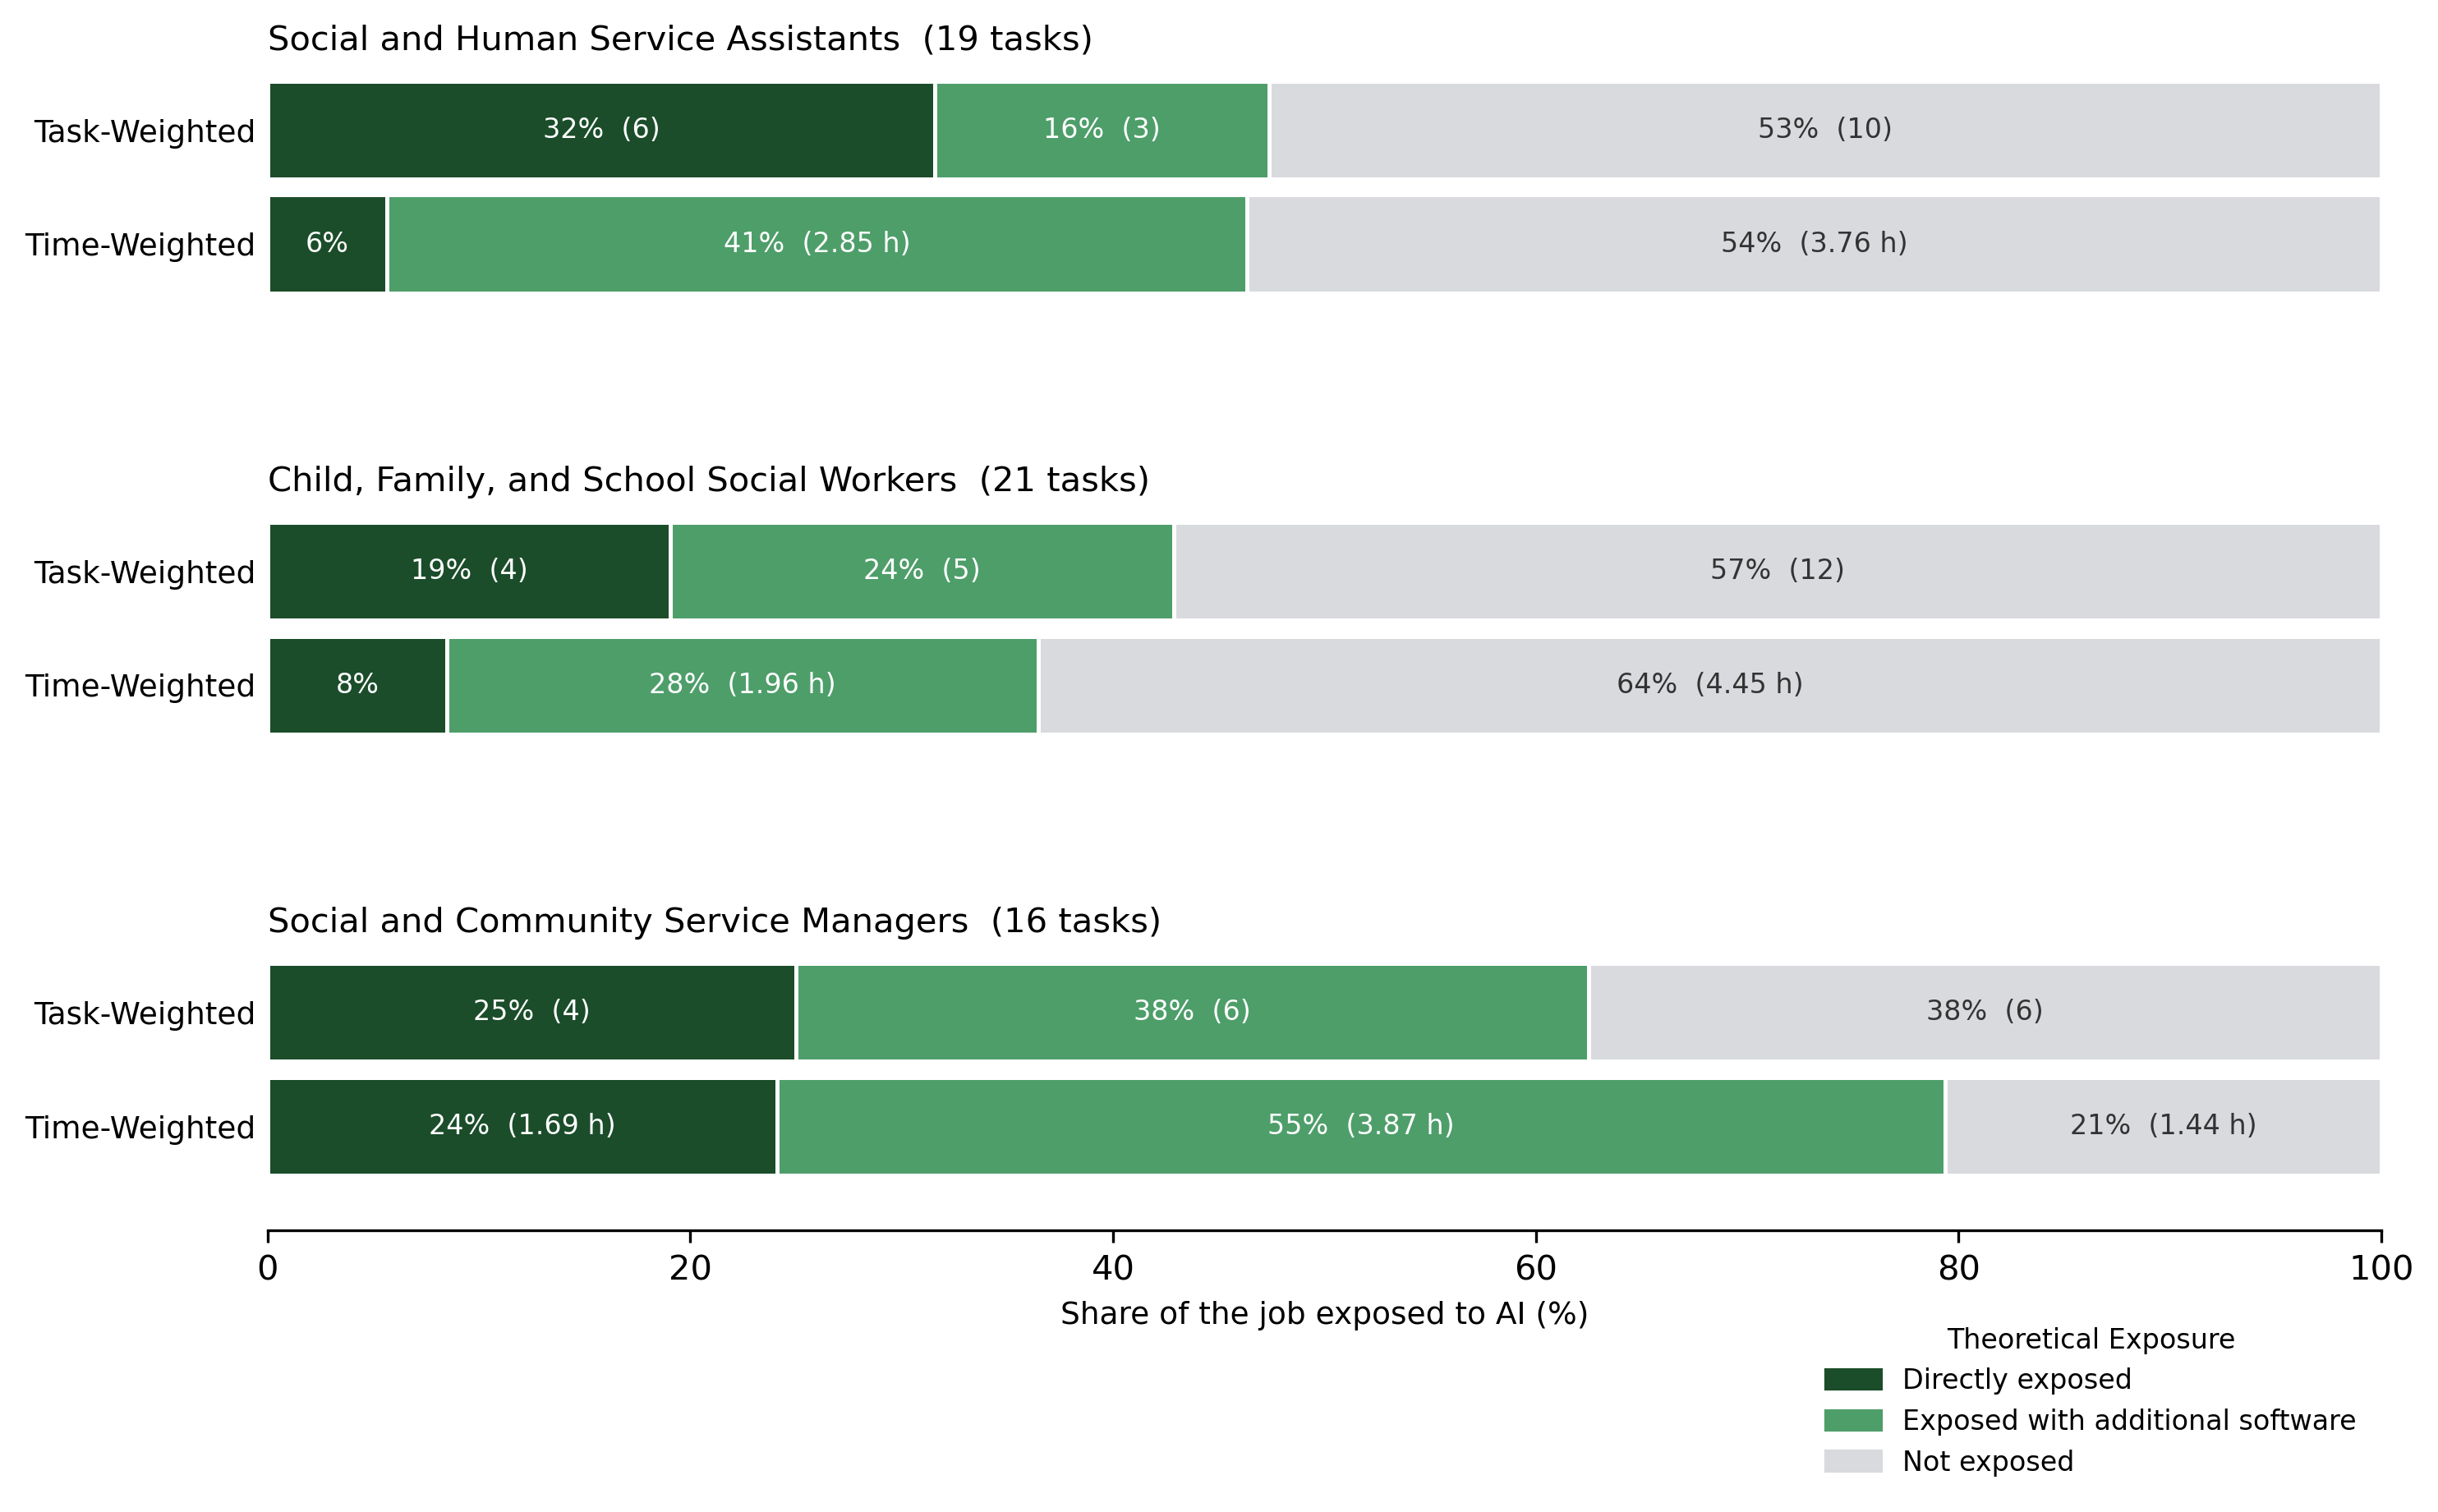
\includegraphics[width=1.0\textwidth]{figures/fig4_tasks_vs_time.png}
\end{figure}

For Social and Human Service Assistants, a third of tasks are directly exposed, but this translates to only 6 percent of the worker's day (Table 4). The total exposure (direct and partial exposure) is almost the same under both measures: 47 percent of tasks and 46 percent of time. What changes is its composition- a much greater share of the worker's day would require dedicated software in order to completely automate when considering the amount of time to complete tasks. The reason is that the directly exposed tasks are quick to do. The six of them average about 4 minutes a day each, while the three partially exposed (software-dependent) tasks average nearly an hour.

Child, Family, and School Social Workers show the same pattern on a smaller scale. Directly exposed work falls from 19 percent of tasks to 8 percent of time, while partially exposed work rises slightly, from 24 to 28 percent. The total exposure of Child, Family, and School Social workers falls from 43 to 36 percent when time-weighting is incorporated.

Social and Community Service Managers show a different pattern. Their directly exposed share is nearly the same under both exposure metrics. Their partially exposed share rises from 38 to 55 percent, because one task, "Implement and evaluate staff, volunteer, or community training programs," takes up 41 percent of the day. The total exposure of managers is therefore higher when time-weighting is considered, rising from 63 percent of tasks to 79 percent of time.

\subsection{Observed use}

Observed AI use, measured from Claude conversations in the workplace, reaches very few of the tasks in these occupations. Of the 56 tasks examined, four show work-related use above the reporting threshold, and together they account for a small share of the working day (Table 5).

\begin{table}[!htbp]
\tablesize
\caption*{\textbf{Table 5.} Tasks with observed AI use.}
\begin{tabularx}{\textwidth}{@{}>{\raggedright\arraybackslash}p{3.4cm} >{\raggedright\arraybackslash}X >{\raggedleft\arraybackslash}p{1.5cm} >{\raggedright\arraybackslash}p{2.5cm}@{}}
\toprule
Occupation & Task & Minutes per day & Exposure category \\
\midrule
Social and Human Service Assistants & None & 0 & n/a \\
Child, Family, and School Social Workers & Conduct social research & 6 & Partially exposed \\
Social and Community Service Managers & Research and analyze member or community needs to determine program directions and goals & 26 & Partially exposed \\
& Evaluate the work of staff and volunteers to ensure that programs are of appropriate quality and that resources are used effectively & 15 & Not exposed \\
& Prepare and maintain records and reports, such as budgets, personnel records, or training manuals & 12 & Partially exposed \\
\bottomrule
\end{tabularx}
\tablenote{\emph{Note:} Observed AI use from Massenkoff and McCrory (2026).}
\end{table}

None of the 19 tasks performed by Social and Human Service Assistants show observed use. For Child, Family, and School Social Workers, only 1 task does, and it occupies 6 minutes of the workday. For Social and Community Service Managers, three tasks of 16 show use. They occupy 53 minutes (about 13 percent of the mangers' workday).

The tasks with recorded use are not the ones rated as directly exposed. Three of the four are rated as partially exposed and one as not exposed. None of the 14 directly exposed tasks across the three occupations show recorded use.

\subsection{Worker hours}

Multiplied across each occupation's workforce, directly exposed time is modest for frontline staff and largest for managers (Table 6).

\begin{table}[!htbp]
\tablesize
\caption*{\textbf{Table 6.} Daily worker hours by exposure category.}
\begin{tabularx}{\textwidth}{@{}>{\raggedright\arraybackslash}X r >{\raggedleft\arraybackslash}p{2.2cm} >{\raggedleft\arraybackslash}p{2.3cm} >{\raggedleft\arraybackslash}p{2.1cm}@{}}
\toprule
Occupation & Total hours & Directly exposed hours & Partially exposed hours & Not exposed hours \\
\midrule
Social and Human Service Assistants & 253,750 & 14,273 (6\%) & 103,338 (41\%) & 136,139 (54\%) \\
Child, Family, and School Social Workers & 97,580 & 8,269 (8\%) & 27,308 (28\%) & 62,002 (64\%) \\
Social and Community Service Managers & 95,760 & 23,074 (24\%) & 52,924 (55\%) & 19,762 (21\%) \\
\bottomrule
\end{tabularx}
\end{table}

Social and Human Service Assistants work about a combined 253,750 hours a day, of which about 14,300 are spent on directly exposed tasks. For Child, Family, and School Social Workers the figure is about 8,300 of 97,600 hours across the workforce. Social and Community Service Managers account for the most directly exposed time, about 23,100 hours a day, although there are more than twice as many assistants (36,250 assistants) than managers in this sector (13,680 managers).

Because a directly exposed task is one that AI could complete in half the time or less, the minimum saving is half of these figures: about 7,100 hours a day for assistants, 4,100 for social workers, and 11,500 for managers.

In every occupation, the share of partially exposed time is much greater. For assistants it is about 103,300 hours a day, seven times their directly exposed time. I do not estimate a saving for partially exposed time, since it depends on software that has not been built.

\subsection{Sensitivity to rating source}

All results shown in this analysis were using human estimates of time to complete tasks. Here, the analysis is repeated using time to complete estimates judged by GPT-4 in order to test the sensitivity of the results. This sensitivity analysis leaves the frontline findings intact but changes the result for managers (Table 7).

\begin{table}[!htbp]
\tablesize
\caption*{\textbf{Table 7.} Daily hours by exposure category under human and GPT-4 ratings.}
\begin{tabularx}{\textwidth}{@{}>{\raggedright\arraybackslash}X >{\raggedright\arraybackslash}p{3.1cm} >{\raggedright\arraybackslash}p{3.2cm} >{\raggedright\arraybackslash}p{2.9cm}@{}}
\toprule
Occupation & Directly exposed (human / GPT-4) & Partially exposed (human / GPT-4) & Not exposed (human / GPT-4) \\
\midrule
Social and Human Service Assistants & 0:24 / 0:43 & 2:51 / 3:56 & 3:45 / 2:21 \\
Child, Family, and School Social Workers & 0:36 / 0:35 & 1:58 / 1:31 & 4:27 / 4:54 \\
Social and Community Service Managers & 1:41 / 0:12 & 3:52 / 5:45 & 1:27 / 1:03 \\
\bottomrule
\end{tabularx}
\tablenote{\emph{Note:} Both sets of ratings are from Eloundou et al. (2024).}
\end{table}

The two sets of ratings agree on 29 of the 56 tasks (52 percent). They disagree most about which tasks are directly exposed. Human judges rated 14 tasks as directly exposed- the GPT-4 judge was more cautious: it agreed on only 3 of them, rating 9 of the others as partially exposed and 2 as not exposed.

For the two frontline occupations, the main finding holds under either rating. Directly exposed time is under an hour a day: 24 minutes according to a human judge and 43 minutes with a GPT-4 judge for Social and Human Service Assistants, and 36 and 35 minutes under both judges for Child, Family, and School Social Workers. In both occupations, partially exposed time is several times larger than directly exposed time whether a human rating or GPT-4 rating is used.

For Social and Community Service Managers, the result depends on the rating. Directly exposed time is 1 hour 41 minutes when judged by humans and 12 minutes when judged by GPT-4, with the difference moving almost entirely into the partially exposed category. The two sets of judges agree on the exposure category for only 5 of the 16 managerial tasks.
